%*******************************************************************************
%****************************** Second Chapter *********************************
%*******************************************************************************

\chapter{Thiết kế và hiện thực \newline sản phẩm móc khóa thông minh - Smart Keyring}

\ifpdf
    \graphicspath{{Chapter2/Figs/Raster/}{Chapter2/Figs/PDF/}{Chapter2/Figs/}}
\else
    \graphicspath{{Chapter2/Figs/Vector/}{Chapter2/Figs/}}
\fi


%\section[Short title]{Reasonably long section title}
\section{Thiết kế sản phẩm}
% Uncomment this line, when you have siunitx package loaded.
%The SI Units for dynamic viscosity is \si{\newton\second\per\metre\squared}.
\subsection{Tính năng sản phẩm}
\label{feature}
Sản phẩm Smart Keyring sẽ có các tính năng cơ bản như:

• Báo hiệu khi mất kết nối: hỗ trợ việc cảnh báo người tránh bỏ quên 1 trong 2 thiết bị.

• Báo hiệu khi kích hoạt chức năng tìm kiếm: cho phép người dùng định vị thiết bị còn lại trong phạm vi kết nối.

• Hai chế độ báo hiệu bằng âm thanh hoặc ánh sáng đèn led hoặc cả 2: mục đích sử dụng trong nhiều trường hợp khác nhau như đêm tối, không gian yên tĩnh...

\subsection{Các thiết bị phần cứng}
%TODO các thiệt bị phần cứng, thêm hình vẽ mạch đồ vào
Sử dụng module HM-10 dùng chip CC2541 vì có thể tìm được tại các cửa hàng thiết bị linh kiện
Mo
Atmel
....

\newpage
\section{Hiện thực phần cứng}
\subsection{Mô hình hoạt động}
Dựa theo tính năng sản phẩm ở mục \ref{feature}, mô hình ứng dụng khi bị thất lạc được thế kế như hình \ref{fig: ble}
	\begin{figure}[h]
		\centering    
		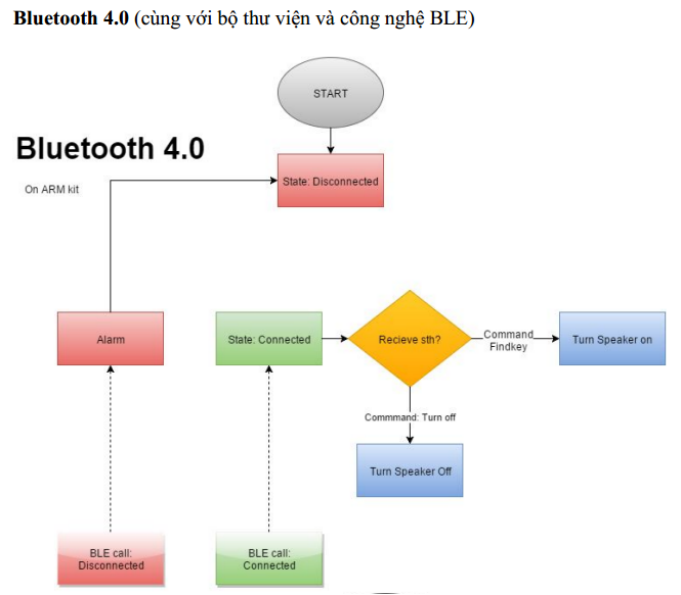
\includegraphics[width=1.0\textwidth]{ble}
		\caption[Sơ đồ hoạt động trên sản phẩm]{Sơ đồ hoạt động của ứng dụng}
		\label{fig: ble}
	\end{figure}
\subsection{Hiện thực}
\newpage
\section{Hiện thực ứng dụng di động trên Android}
\subsection{Mô hình hoạt động}
Dựa theo tính năng sản phẩm ở mục \ref{feature}, mô hình ứng dụng khi bị thất lạc được thế kế như hình \ref{fig: blelost}
	\begin{figure}[h]
		\centering    
		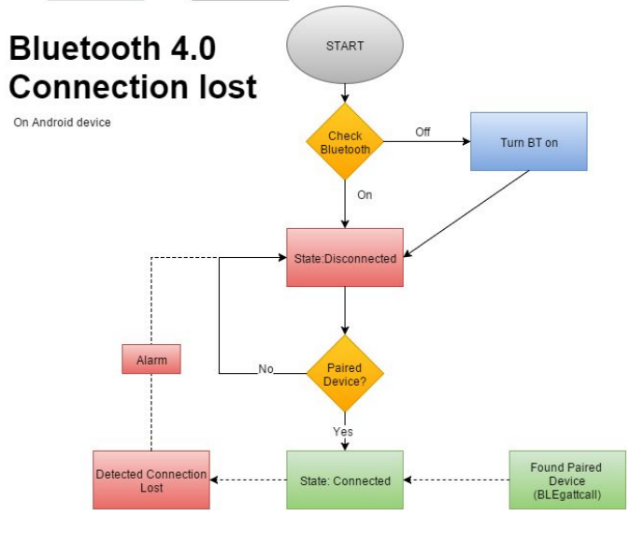
\includegraphics[width=1.0\textwidth]{blelost}
		\caption[Sơ đồ hoạt động trên thiết bị di động]{Sơ đồ hoạt động của ứng dụng}
		\label{fig: blelost}
	\end{figure}
\subsection{Các module trong ứng dụng Android}

